\section{SQL Parser}

\subsection{über den SQL Parser: ZQL}

Auf der Webseite vom \cite{zql1} Projekt ist der Open-Source-Parser ZQL zu finden, welcher in der Lage ist SQL zu parsen und in Datenstrukturen zu überführen. Der Parser selbst ist mit \cite{javacc1} geschrieben, einem  Java-Parsergenerator (zu vergleichen mit dem populärem Unix yacc Generator).

ZQL bietet Unterstützung für \verb|SELECT-|,\verb|INSERT-|,\verb|DELETE-|,\verb|COMMIT-|,\verb|ROLLBACK-|,\verb|UPDATE-| und \verb|SET TRANSACTION-|Ausdrücke. Wichtig für diese Arbeit sind dabei insbesondere \verb|SELECT-| und \verb|UPDATE-|Ausdrücke, sowie -- die leider nicht enthaltenen -- \verb|CREATE TABLE-|Ausdrücke.

\subsection{Funktionsweise des Parsers}

ZQL kennt zwei grundlegende Interfaces \verb|ZExp| und \verb|ZStatement|. 

Das Interface \verb|ZStatement| bildet eine abstrakte Oberklasse für alle möglichen Arten von SQL-Statements. Folgende Klassen implementieren dieses Interface in ZQL:

\begin{itemize}
\item \verb|ZDelete| - repräsentiert ein \verb|DELETE| Statement
\item \verb|ZInsert| - repräsentiert ein \verb|INSERT| Statement
\item \verb|ZUpdate| - repräsentiert ein \verb|UPDATE| Statement
\item \verb|ZLockTable| - repräsentiert ein \verb|SQL LOCK TABLE| Statement
\item \verb|ZQuery| - repräsentiert ein \verb|SELECT| Statement
\end{itemize}

Das Interface \verb|ZExp| bildet eine abstrakte Oberklasse für drei verschiedene Arten von Ausdrücken:

\begin{itemize}
\item \verb|ZConstant| - Konstanten vom Typ \verb|COLUMNAME, NULL, NUMBER, STRING| oder \verb|UNKNOWN|
\item \verb|ZExpression| - Ein SQL-Ausdruck bestehend aus einem Operator und einen oder mehreren Operanden
\item \verb|ZQuery| - Eine \verb|SELECT| Anfrage ist auch ein Ausdruck
\end{itemize}

Da die \verb|SELECT| Anfragen die wohl am häufigsten gebrauchte Form der Anfragen ist, wird sich die Erklärung der Funktionsweise des Parsers beispielhaft auf diese Art der Anfragen beziehen. Wie die anderen Statements geparst werden ist dann analog schnell zu verstehen.

Eine gewöhnliches Select-Statement wird wie folgt vom Parser zerlegt:
\begin{verbatim}SELECT e.name FROM emp e WHERE e.sal > 1000 ORDER BY e.sal DESC\end{verbatim}

\begin{tabular}{ll}
\verb|SELECT e.name| & \textit{Vector} von \textit{ZSelectItem} enthält \verb|e.name| \\ 
\verb|FROM emp e| & \textit{Vector} von \textit{ZFromItem} enthält \verb|emp| mit Alias \verb|e| \\
\verb|WHERE e.sal > 1000| & \textit{ZExpression} mit Operator \verb|>| und Operanden\textit{Vector} der Form \{\verb|e.sal|, \verb|1000|\} \\
\verb|ORDER BY e.sal DESC| & \textit{ZOrderBy}-Objekt mit enthaltenem \verb|ORDER BY| Sortierausdruck und Reihenfolge
\end{tabular}

%TODO: Parsebäume nicht binär
Eine Besonderheit des ZQL-Parsers sind seine Parserbäume. Ein üblicher Syntaxbaum ist binär, wobei die Wurzel den Operator mit der höchsten Priorität darstellt. Alle Teilbäume sind wieder als Ausdrücke zu verstehen, jeweils mit Operator als Wurzelknoten und Operanden als Kindknoten. Dabei kann ein Operand auch ein weiterer Ausdruck sein. Generell wird dabei das Prinzip der Assoziativität benutzt um z.B.: für gleichrangige Operatoren eine Auswertungsreihenfolge festzulegen.

So würde der \verb|WHERE|-Teil von folgender SQL-Anfrage:
\begin{verbatim}
SELECT * FROM emp e WHERE e.sal > 1000 AND e.sal < 2000 AND e.id > 1234
\end{verbatim}

zu folgendem geklammerten Ausdruck:
\begin{verbatim}
(((e.sal > 1000) AND (e.sal < 2000)) AND (e.id > 1234))
\end{verbatim}

\begin{figure}
\label{baum1}
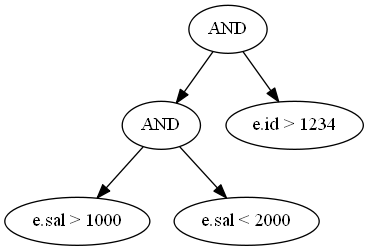
\includegraphics[scale=0.7]{Bilder/where_syntax.png}
\caption{WHERE-Bedingung in üblichen Syntaxbäumen}
\end{figure}

Der ZQL-Parser funktioniert so allerdings nicht. Wird keine spezielle Klammerung benutzt so werden gleichrangige Operatoren nicht assoziativ geklammert, sondern befinden sich auf einer Ebene des Baumes. Somit handelt es sich nicht um einen binären Baum. 

Wir erhalten also aus obigen \verb|WHERE|-Ausdruck:
\begin{verbatim}
((e.sal > 1000) AND (e.sal < 2000) AND (e.id > 1234))
\end{verbatim}

\begin{figure}
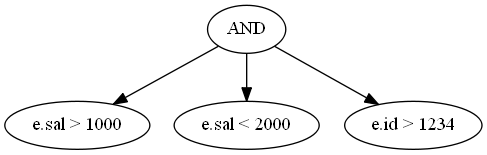
\includegraphics[scale=0.7]{Bilder/with_zql.png}
\caption{WHERE-Bedingung geparst mit ZQL}
\end{figure}

Wie schon erwähnt werden Operanden daher in einer \textit{Vector} Struktur gespeichert.

\subsection{Grenzen des Parsers}

Der Parser kann keine \verb|CREATE TABLE| Statements parsen. Somit ist es im Rahmen dieser Arbeit notwendig, den Parser zu erweitern, damit Tabellen in eigene Datenstrukturen geparst werden können. Für die Arbeit ist es zunächst nur notwendig Name und Datentyp der Spalten in eine interne Datenstruktur zu überführen. Dabei wird nur zwischen Zahlen und Sonstigem (Text) unterschieden. Unser Programm soll in der Lage sein, einfache arithmetische Operationen durchzuführen. Dazu ist das wissen um Datentypen der Variablen von Nöten.

Weiterhin ist der ZQL-Parser nicht in der Lage \verb|JOINS| über die Schlüsselworte \\\verb#ON [LEFT OUTER|RIGHT OUTER|INNER] JOIN# zu realisieren. Der Parser erkennt nur innere \verb|JOINS|, die im \verb|WHERE|-Teil formuliert worden. Das soll für diese Arbeit ohne weitere Bedeutung sein, da dennoch Strategien entwickelt werden, wie man mit derartigen \verb|JOINS| umgeht. Es muss an der Stelle nur erwähnt werden, dass das Programm, welches im rahmen dieser Arbeit entsteht, mit derartigen \verb|JOINS| nicht umgehen kann.

Trotz dieser Einschränkungen sind alle Konzepte, die in dieser Arbeit vorgestellt werden einfach auf jedweden SQL-Parser übertragbar.

%TODO: CREATE TABLE

\section{Java Server Pages}

\subsection{Überblick}

\subsection{Einbettung in JSP}

\subsection{Log}